%class
	\documentclass{beamer}

%template
	\usetheme{HannoverSalman}
	\setbeamertemplate{navigation symbols}{}
	%\setbeamertemplate{footline}{\centering{\insertframenumber/\insertpresentationendpage}}
	%\setbeamertemplate{footline}{\hspace*{.5cm}\scriptsize{\hfill\insertframenumber\hspace*{.5cm}}} 


%packages
	\usepackage{amsmath, amssymb, graphicx,cancel}
	\usepackage[absolute,overlay]{textpos}
	\usepackage{subfigure}
	\usepackage{caption}\captionsetup{labelformat=empty,labelsep=none}
	\usepackage{geometry}
	\geometry{verbose}
	\usepackage{color}
	\usepackage{xmpmulti}
	\usepackage[3D]{movie15}
	\usepackage{hyperref}
%	\usepackage{bookmark}
	\usepackage[open,openlevel=4,atend]{bookmark}
	%\bookmarksetup{color=blue}
	\usepackage{multirow}
	\usepackage[style=numeric,defernumbers, authoryear]{biblatex}
	%\usepackage[square,sort]{natbib}
	%\usepackage{fancyhdr}%\pagestyle{fancy} 

	
	\hypersetup{bookmarksdepth = 4}


%citations files
	\bibliography{MyCitations}

%logoCSIPCPL
    \setlength{\TPHorizModule}{1mm}
    \setlength{\TPVertModule}{1mm}
    \newcommand{\logoCSIPCPL}
    {
    	\begin{textblock}{1}(100,2) %(100,85)  for bottom
    		
\includegraphics[width=1.5cm]{figs/logo_CSIP}
    	\end{textblock}
    	
	\begin{textblock}{1}(117,1) %(117,85)  for bottom
    		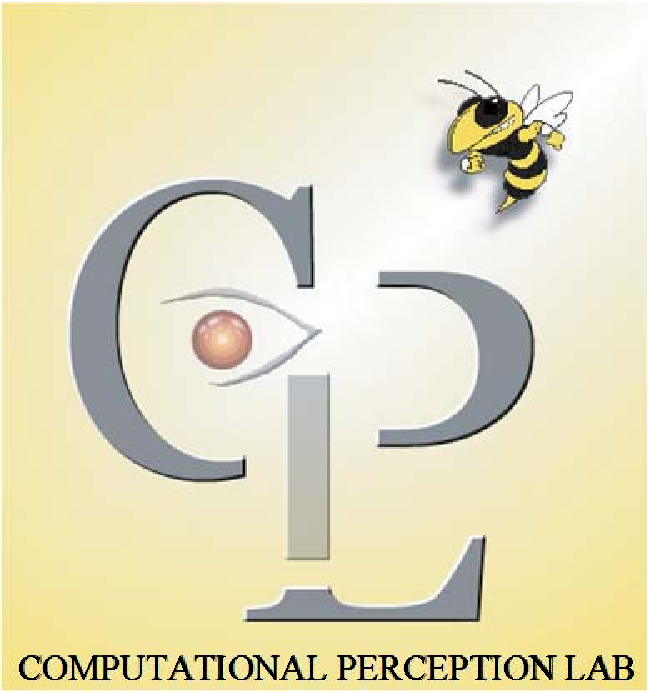
\includegraphics[width=1.0cm]{figs/logo_CPL}
    	\end{textblock} 
    }

%logo evolution
    \newcommand{\logoEvolution}
    {    	
	\begin{textblock}{1}(110,1) %(117,85)  for bottom
    		\includegraphics[width=0.65in]{figs/logo_evolution.pdf}
    	\end{textblock} 
    }

%logo Qualcomm
    \newcommand{\logoQualcomm}
    {
    	\begin{textblock}{1}(110,2) %(100,85)  for bottom
    		\includegraphics[width=1.5cm]{figs/logo_qualcomm.jpg}
    	\end{textblock}
    }
%logo Qualcomm (long)
    \newcommand{\logoQualcommllong}
    {
    	\begin{textblock}{1}(0,0) 
    		\includegraphics[width=1.25in]{figs/logo_qualcomm_long.jpg}
    	\end{textblock}
    }

%logo Tech Tower
    \newcommand{\logoTechTower}
    {
    	\begin{textblock}{1}(0,0) 
    		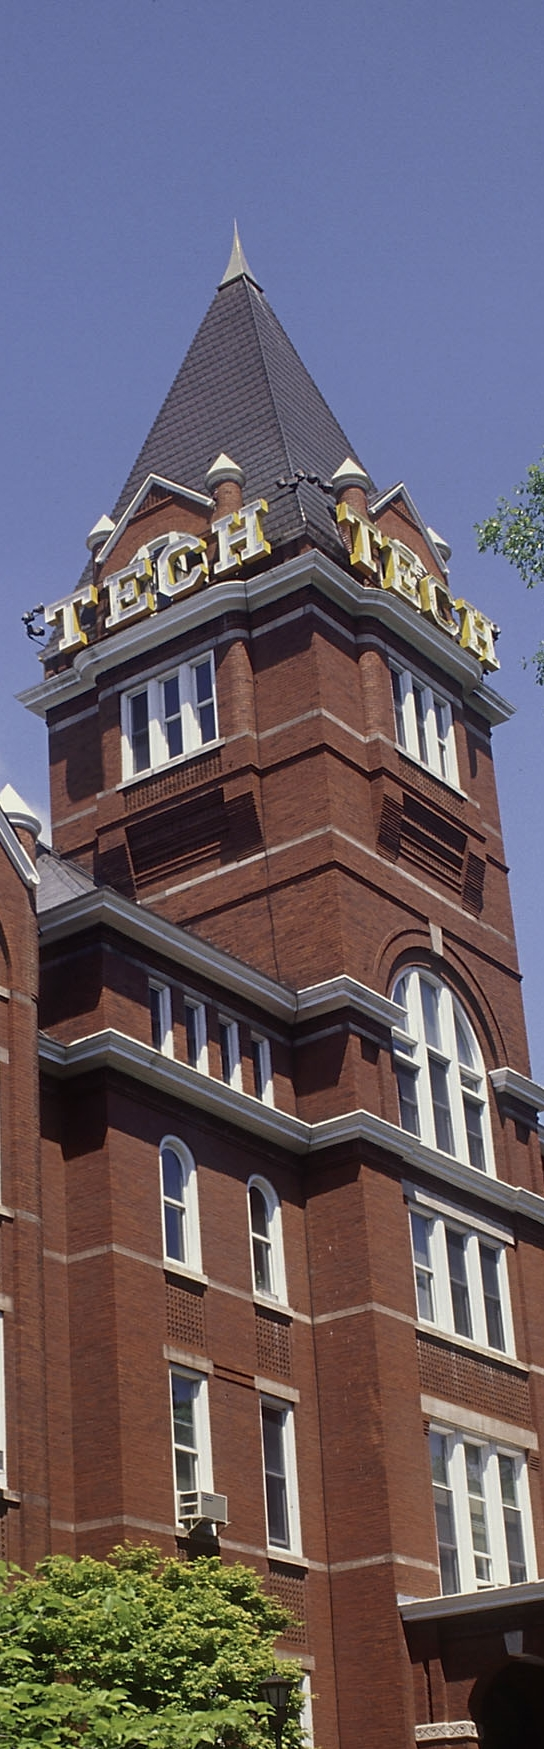
\includegraphics[width=1.25in]{figs/logo_TechTower.jpg}
    	\end{textblock}
    }

%logo tree
    \newcommand{\logoTree}
    {
    	\begin{textblock}{1}(0,0) 
    		\includegraphics[width=1.25in]{figs/logo_tree.jpg}
    	\end{textblock}
    }
%page numbers
    \newcommand{\mypagenum}
    {
    	\begin{textblock}{1}(1,94) 
		{\tiny \color[rgb]{0.2,0.2,1}\insertframenumber} %\insertframenumber,\insertpresentationendpage, \inserttotalframenumber
    	\end{textblock}
    }
%my footnote citation
	\newcommand{\myFootnoteCitation}[2]
	{
		\footnote{\tiny \citeauthor{#1}, \emph{#2}, \citeyear{#1}.}  %\citeauthor{#1}, \citetitle{#1}, #2 \citeyear{#1}.
	}
%my refer to citation
	\newcommand{\mycite}[1]
	{
		\emph{\citeauthor{#1} (\citeyear{#1})}
	}
%my footnote website citation
	\newcommand{\myFootnoteWebsiteCitation}[1]
	{
		\footnote{\tiny \citeauthor{#1}}
	}

\let\thefootnote\relax\footnotetext{Footnotetext without footnote mark}


%section underline
%\newcommand{\tmpsection}[1]{}
%\let\tmpsection=\section
%\renewcommand{\section}[1]{\tmpsection{\underline{#1}}}



%commands
	\newcommand{\likelihood}{p(Z_k| x_k) }						%likelihood
	\newcommand{\prior}{p(x_k)  } 								%prior
	\newcommand{\posterior} {p(x_k| Z_k)}						%posterior
	\newcommand{\prediction} {p(x_k| Z_{k-1})}					%prediction
	\newcommand{\update} {p(x_k|Z_k)}							%update
	\newcommand{\observations} {p(Z_k)}						%observations
	\newcommand{\prevobservations} {p(Z_{k-1})}				%previous observations
	\newcommand{\dxpk} {dx_{k-1}}							%dx_{k-1}
	\newcommand{\ChapKolm}{\int{p(x_k| x_{k-1})p(x_{k-1}|Z_{k-1})} \dxpk} %Chapman Kolmogorov

	%algorithm specific: JPDAF
	\newcommand{\likelihoodJPDAF}{p(Z_k| \chi, m, Z_{k-1}) }		%1. likelihood
	\newcommand{\priorJPDAF}{p(\chi|m, Z^{k-1}} 				%2. prior	
	\newcommand{\observationsJPDAF} {p(Z_k}					%3. observations
	\newcommand{\posteriorJPDAF} {p(\chi| Z_k)}					%4. posterior

%environments
	\newenvironment{changemargin}[2]
	{
	  	\begin{list}{}
		{
			\setlength{\topsep}{0pt}%
			\setlength{\leftmargin}{#1}%
			\setlength{\rightmargin}{#2}%
			\setlength{\listparindent}{\parindent}%
			\setlength{\itemindent}{\parindent}%
			\setlength{\parsep}{\parskip}%
		}
	  	\item[]
		}
		{\end{list}
	}
%figures

%colors
\definecolor{darkgreen}{rgb}{0,0.5,0}

%personal details
	\author{Salman Aslam}
	\institute{Advisor, Dr Christopher Barnes (ECE)\\Co-advisor, Dr Aaron Bobick (CoC)\\Georgia Institute of Technology}
	\date{}

\begin{document}
%####################################################################################################
\title{Computer Vision}
%####################################################################################################
\begin{frame}\logoTree
	\institute{}
	\titlepage
\end{frame}


%####################################################################################################
\section{Introduction}
%####################################################################################################
\begin{frame}\frametitle{Probability vs inference}\logoEvolution\mypagenum
	A concise course in statistical inference (Larry Wasserman)
	\begin{figure}
		\includegraphics[width=0.9\textwidth]{figs/PRML_inference_probability.png}
	\end{figure}
\end{frame}

\begin{frame}\frametitle{Notation}\logoEvolution\mypagenum
	\begin{figure}
		\includegraphics[width=0.9\textwidth]{figs/CV_ML_notation.pdf}
	\end{figure}
\end{frame}



%####################################################################################################
\section{Active Appearance Models}
%####################################################################################################

\begin{frame}\frametitle{Active Appearance Models}\logoCSIPCPL\mypagenum
	\begin{itemize}
		\item basis for shape representation
		\item model constrained to generate shapes similar to those in training set		
		\item modeling how different labeled points tend to move together as shape varies
		\item training set is aligned
		\item $x_i$ is a vector describing the $n$ points of the $i$-th shape
			\begin{equation}
			x_i = \{x_{i0}, y_{i0}, x_{i1}, y_{i1}, \ldots x_{in-1}, y_{in-1}\}
			\end{equation}
		\item $2n$x$2n$ covariance matrix is then computed
		\item principal axes of the ellipsoid give the modes of variation of the points of the shape
	\end{itemize}
{\footnotetext{\tiny T.F. Cootes, C.J. Taylor, D.H. Cooper, and J. Graham, "Active shape models-their training and application," \emph{Computer Vision and Image Understanding}, vol. 61, no. 1, pp. 38 -59, 1995.}}
\end{frame}



%#######################################################################
\section{3D}
%#######################################################################

\begin{frame}\frametitle{Theory}\logoEvolution\mypagenum
	The following slides contain some slides on related theoretical issues.
\end{frame}

%====================================================
\subsection{\ \ - Acquisition, processing, display}
%====================================================
\begin{frame}\frametitle{Acquisition, processing and display}
	\begin{figure}
		\includegraphics[width=3.5in]{figs/3D_acquisition_and_display_blockDiagram.pdf}
	\end{figure}
%\cite{1838_JNL_Stereo_Wheatstone,1989_JNL_StructureFromStereo_Dhond,2001_JNL_Future3Dvideo_Ollis,2003_JNL_SurveyStereo_Brown,2005_JNL_SpaceTimeStereo_Davis,2005_WHITE_Survey3Ddisplay_May,2006_CNF_2D3D_Knorr,2006_CNF_Survey2D3D_Tam,2007_CNF_DMcolorSegmentation_Chang,2007_JNL_2D3Drealtime_Ideses,2008_CNF_PoseTracking_Wagner,2010_TECH_2Dto3D_Zhang}
%\cite{2010_CNF_HMMRVQ_Aslam,2010_CNF_TrkRVQ_Aslam}
\end{frame}		
		

%====================================================
\subsection{\ \ - 1 camera}
%====================================================
\begin{frame}\frametitle{3D world $\rightarrow$ 2D camera}\logoEvolution\mypagenum
	\begin{figure}
		\includegraphics[height=0.9\textheight]{figs/3D_1_camera_equations.pdf}
	\end{figure}
\end{frame}





%====================================================
\subsection{\ \ - 2 cameras}
%====================================================
\begin{frame}\frametitle{Notation}\logoEvolution\mypagenum
	\begin{figure}		
		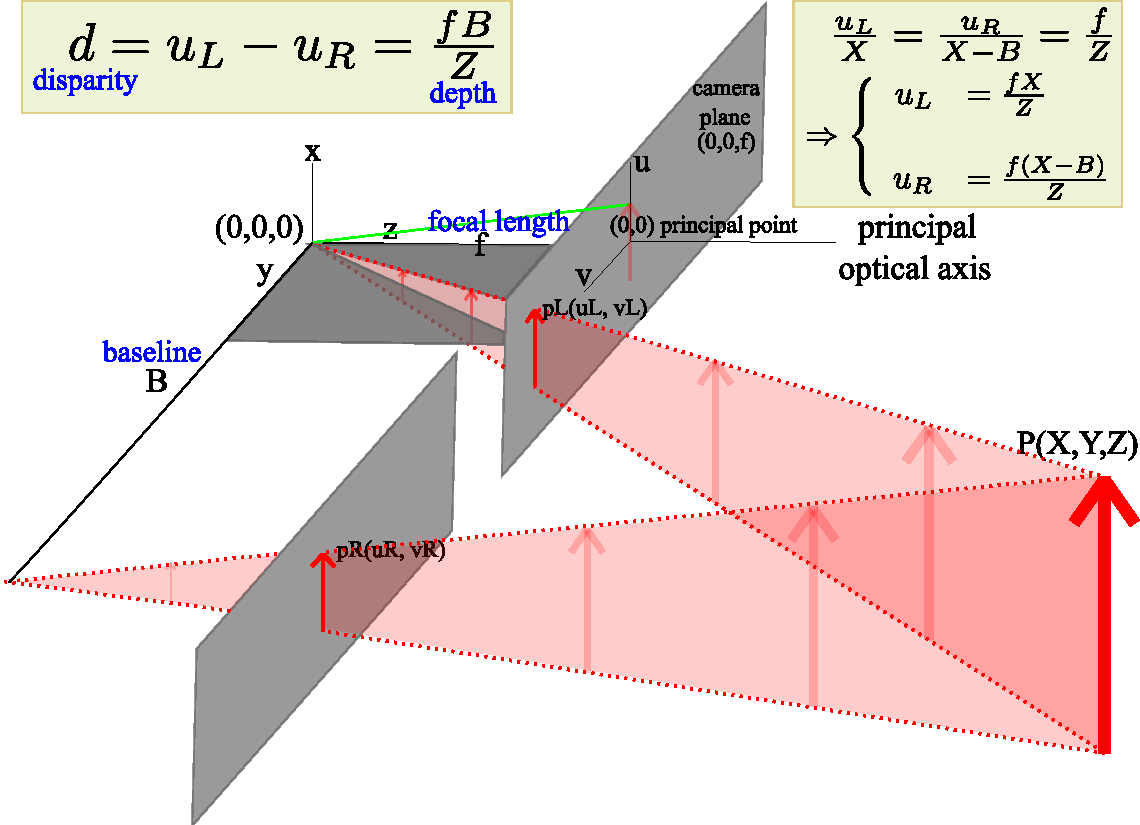
\includegraphics[width=3.5in]{figs/3D_2_cameras_blockDiagram.pdf}
	\end{figure}
\end{frame}	


%====================================================
\subsection{\ \ - display .u3d file}
%====================================================

\begin{frame}
\frametitle{3D (display .u3d file)}
\framesubtitle{MakeHuman $\rightarrow$ Blender $\rightarrow$ .obj $\rightarrow$ DAZ Studio $\rightarrow$ .u3d}
\mypagenum
%\includemovie[poster, label=my_label, 3Dcalculate, 3Droo=3000, toolbar, 3Djscript=turntable.js]
%{0.75\textwidth}{0.75\textwidth}{figs/human_original.u3d}\\
\includemovie[poster, label=my_label, 3Dcalculate, 3Droo=3000, toolbar]
{0.75\textwidth}{0.75\textwidth}{figs/human_original.u3d}\\
\movieref[human_original]{my_label}{}
\end{frame}


%%==========================================================
%\section{Perspective Projection}
%%==========================================================
%
%\textbf{Camera model.} Each 3D point is projected along viewing rays
%onto the image plane. Depending on the chosen camera model, these
%viewing rays are parallel (parallel projection or orthographic
%projection), or they all intersect in a single point, the optical
%center (perspective projection).
%
%For orthographic projection, the image coordinates $(x,y)$ are
%directly determined from the 3D object point $(x_p, y_p, z_p)$
%according to
%
%\begin{equation}\label{eqn: OrthographicProjection}
%\begin{split}
%x=x_p \\
%y=y_p
%\end{split}
%\end{equation}
%
%Note that the depth of the object point has no influence on the
%resulting image coordinate.  All rays coming from the 3D object are
%assumed to be parallel which is a good approximation for cameras
%with a large focal length corresponding to a small viewing angle.
%Due to the linear mapping of the coordinates in Equation \ref{eqn:
%OrthographicProjection}, the use of this projection model leads to
%simpler algorithms for the estimation of motion parameters from 2D
%images.
%
%The perspective projection uses a non-linear mapping between 3D and
%2D coordinates given by
%
%\begin{equation}\label{eqn: PerspectiveProjection1}
%\begin{split}
%\frac{x}{x_p}= \frac{z}{z_p} \\
%\frac{y}{y_p}= \frac{z}{z_p}
%\end{split}
%\end{equation}
%
%Here $z_p$ is equal to the distance between the optical center and
%the image plane, and can be replaced with $f$
%
%\begin{equation}\label{eqn: PerspectiveProjection2}
%\begin{split}
%x= f \frac{x_p}{z_p} \\
%y =f \frac{y_p}{z_p}
%\end{split}
%\end{equation}
%
%
% \textbf{Pinholes.}  The first models of \emph{camera obscura},
%literally dark chamber, invented in the 16th century did not have
%lenses but used a \emph{pinhole} to focus light rays onto a wall or
%translucent plate and demonstrate the laws of perspective discovered
%a century earlier by Brunelleschi (1377  April 15, 1446)
%
%\textbf{Lenses.}  Pinholes were replaced by more sophisticated
%lenses as early as 1550.
%
%\textbf{Imaging surface.}  For normal cameras, it is generally a
%rectangle. For panoramic cameras and the eye, it is spherical.
%
%\textbf{image plane.}
%
%\textbf{Hyperspectral sensors.}
%
%\textbf{Pinhole perspective projection model or Central Perspective
%Projection Model.}  This model creates inverted images.  Two
%byproducts of this model are that far objects appear smaller than
%closer ones.
%
%\textbf{virtual image.} Convenient to consider it in front of the
%pinhole at the same distance from it as the actual image plane.
%
%\textbf{projection.} The \emph{projections} of two parallel lines
%lying in some plane $\Pi$ appear to converge on a horizon line $H$.
%The horizon line is formed by the intersection of the image plane
%with a plane passing through the pinhole and parallel to $Pi$.
%
%Think of this, where the parallel lines meet at a far off distance,
%you have a pinhole.  Well, since there is a pinhole only over there,
%these lines will definitely meet at the pinhole.
%
%I think the reason is as follows:  when you look straight, you are
%looking at a point.
%
%Another way.  Suppose your two eyes could operate separately and
%they were far apart, and you bend down to the level of the lines, so
%that one could look "down" one line with one eye, and look down the
%other line with the other eye.  Now, both lines would always remain
%parallel.
%
%Now you start getting up, you are at the center of both lines, and
%your eyes are normal again, so they look at one point.  At one
%point, light rays from both lines come, and you feel that the lines
%are intersecting.
%
%\textbf{optical axis.} $\bot$ to image plane passing through
%pinhole.
%
%\textbf{image center.} point at which optical axis hits image plane.
%%%%%%%%%%%%%%%%%%%%%%%%%%%%%%%%%%%%%%%%%%%%%%%%%%%%%%%%%%%%%%%%%%%%%%%%%
%
%
%
%
%
%
%%==========================================================
%\subsection{Affine Projection : Weak projection}
%%==========================================================
%
%%==========================================================
%\subsection{Affine Projection : Orthographic projection}
%%==========================================================
%
%%==========================================================
%\subsection{Homogeneous Coordinates}
%%==========================================================
%In a homogeneous system, a vertex $V(x,y,z)$ is represented as
%
%\begin{equation}
%V(wX, wY, wZ, w)
%\end{equation}
%
%for any scale factor, $w \neq 0$.  The 3D Cartesian coordinate
%representation is then:
%
%\begin{equation}
%\begin{split}
%x=X/w \\
%y=Y/w \\
%z=Z/w
%\end{split}
%\end{equation}
%
%To denote a point, w=1, and its matrix notation is
%
%\begin{equation}
%\begin{pmatrix}
%x \\
%y \\
%z \\
%1
%\end{pmatrix}
%\end{equation}
%
%%==========================================================
%\subsection{Translation}
%%==========================================================
%Translation of a point can be defined as:
%\begin{equation}
%\begin{pmatrix}
%x' \\
%y' \\
%z' \\
%1
%\end{pmatrix}
%=
%\begin{pmatrix}
%1 & 0 & 0 & T_x \\
%0 & 1 & 0 & T_y \\
%0 & 0 & 1 & T_z \\
%0 & 0 & 0 & 1
%\end{pmatrix}
%*
%\begin{pmatrix}
%x \\
%y \\
%z \\
%1
%\end{pmatrix}
%\end{equation}
%
%%==========================================================
%\subsection{non-Euclidean Geometry}
%%==========================================================
%(Forsyth and Ponce, 20)
%Euclid wrote 5 axioms (he called them postulates).  The first 4
%postulates are so self-evident that they clearly ought to be
%satisfied by anything worthy of the name "geometry".  The fifth
%postulate, the parallel postulate says that for any line L and any
%point P not on L, there exists a unique line that is parallel to L
%(never meets L) and passes through P.   For centuries,
%mathematicians tried to prove the 5th postulate using the first 4
%but failed.  Now, it has been realized that this postulate is
%independent of the first 4 and you get a perfectly consistent system
%even if you assume that the parallel postulate is false.  This means
%that it is possible to assign meaning to the terms "point" and
%"line" in such a way that they satisfy the first four postulates but
%not the parallel postulate.  These are called non-Euclidean
%geometries.
%
%\footnote{http://www.math.toronto.edu/mathnet/questionCorner/projective.html}.
%%%%%%%%%%%%%%%%%%%%%%%%%%%%%%%%%%%%%%%%%%%%%%%%%%%%%%%%%%%%%%%%%%%%%%%%%
%
%
%
%
%
%%==========================================================
%\subsection{Euclidean Geometry }
%%==========================================================
%(Forsyth and Ponce, 20)
%
%%==========================================================
%\subsection{Affine geometry}
%%==========================================================
% (Forsyth and Ponce, 253)
%Affine Geometry is, roughly speaking, what is left after all ability
%to measure lengths, areas and angles has been removed from Euclidean
%geometry.  The concept of parallelism remains, however, as well as
%the ability to measure ratio of distances between collinear points.
%Giving a rigorous axiomatic introduction to affine geometry would be
%out of place here.
%
%
%%==========================================================
%\subsection{Projective geometry}
%%==========================================================
%(Forsyth and Ponce, 253)
%Projective geometry is not really a typical non-Euclidean geometry,
%but it can still be treated as such.
%
%In the axiomatic approach, projective geometry means any collection
%of things called "points"  and things called "lines" that obey the
%first four basic properties that points and lines in a familiar flat
%plane do, but which instead of the parallel postulate, satisfy the
%following opposite property instead:
%
%The projective axiom: Any two lines intersect (in exactly one
%point).
%
%Using only this statement, together with the other basic axioms of
%geometry, one can prove theorems about projective geometry.  Many of
%them are the same as ordinary geometry, the big difference is that
%there is no such thing as a pair of parallel, non-intersecting lines
%in projective geometry.
%
%One interesting fact worth mentioning is that in projective
%geometry, points and lines are completely interchangeable.  That is,
%any statement about points and lines would still be true even if you
%replaced all occurrences of the word "point" with the word "line",
%and vice versa.  For instance, the basic axiom that "for any two
%points, there is a unique line that intersects both these points"
%which turned around becomes, "for any two lines, there is a unique
%point that intersects (ie lies on) both those lines".
%
%Each point of projective geometry is a line passing through the
%origin in 3D space.  So projective geometry can be thought of as the
%collection of all lines through the origin in 3D space.  The
%distance between 2 points can be thought of as the angle between the
%corresponding lines.
%
%A line in projective geometry is really a family of lines through
%the origin in 3D space.
%
%
% The means of measurement available in
%projective geometry are even more primitive than those available in
%affine geometry. The affine notions of ratios of lengths along
%parallel lines and in fact, the notion of parallelism are gone.  The
%concepts of points, lines and plains remain, however, as well as a
%new, weaker scalar measure of the arrangement of collinear points -
%the cross-ratio. As in the affine case, a rigorous axiomatic
%introduction to projective geometry would be out of place here.
%
%Take each line of Euclidean geometry and add to it one extra object,
%called a "point at infinity".  For parallel lines, add the same
%object so that the extended lines intersect.  For non-parallel
%lines, add a different object so that the extended lines do not
%intersect more than once).
%
%The points of projective space are the points in Euclidean geometry
%together with these additional objects.
%
%%==========================================================
%\subsection{Points at infinity}
%%==========================================================
%
%The projective space $\mathbb{P}^n$ can be viewed as the union of
%the usual space $\mathbb{R}^n$ and the set of points at infinity.
%The neat thing about this formalism is that the points at infinity
%are not special and are treated just like any other point.
%
%\textbf{Example.}  In the projective plane, there is one point at
%infinity for each direction in the plane.  $(1,0,0)^T$ is associated
%with the horizontal direction, $(0,1,0)^T$ is associated with the
%vertical direction, and so on.
%
%%==========================================================
%\subsection{Euclidean vs Projective Geometry}
%%==========================================================
%
%Euclidean Geometry is based on the 5 basic postulates of Euclid.
%These postulates are quite basic and say things like, "2 points can
%be joined to create a line", etc.  Here we are interested in the 5th
%postulate which basically states that two parallel lines will never
%intersect.
%
%Projective Geometry, introduced to better understand perspective
%drawing, differs from Euclidean Geometry in this 5th postulate.  In
%this way, it is a form of non-Euclidean Geometry.
%
%\textbf{2D Projective Geometry.}  In 2D projective geometry, 2 lines
%will \emph{always} intersect at a point \footnote{Parallel lines
%will intersect at infinity.}.  The following equation is used to
%represent points and lines:
%
%\begin{equation}
%ax + by + cw = 0
%\end{equation}
%
%In this equation, 3 coordinate points define both a point and a
%line.  This is discussed further in the following lines.
%
%\textbf{Equation of point in 2D projective geometry}. If $(x,y,w)$
%are given, we have an equation for a point.  You can optionally
%divide $(x,y,w)$ by $w$ to get $(x/w,y/w,w/w)$.  Why would you want
%to do this?  Well, if $w=0$, then dividing by 0 shows that the point
%lies at infinity\footnote{This could be the case if you are
%computing the intersection of two parallel lines.}. The point formed
%by the intersection of two lines $(a_1, b_1, c_1)$ and $(a_2, b_2,
%c_2)$, can be computed using
%
%\begin{equation}
%\begin{pmatrix}
%\hat{i} & \hat{j}   &   \hat{k} \\
%a_1     & b_1       &   c_1 \\
%a_2     & b_2       &   c_2
%\end{pmatrix}
%\end{equation}
%
%
%\textbf{Equation of line in 2D projective geometry}. If $(a,b,c)$
%are given, we have an equation for a line.  Also, just substitute
%$w=1$.  If the equation of the line is of the form $(0,0,w)$, then
%the line lies at infinity.  The line formed by the intersection of
%two points $(x_1, y_1, z_1)$ and $(x_2, y_2, z_2)$, can be computed
%using
%
%\begin{equation}
%\begin{pmatrix}
%\hat{i} & \hat{j}   &   \hat{k} \\
%x_1     & y_1       &   z_1 \\
%x_2     & y_2       &   z_2
%\end{pmatrix}
%\end{equation}
%
%
%\textbf{3D Projective Geometry.}  In 3D projective geometry, 3
%planes will \emph{always} intersect at a point \footnote{Parallel
%planes will intersect at infinity.}.  The following equation is used
%to represent points and planes:
%
%\begin{equation}
%ax + by + cz + dw = 0
%\end{equation}
%
%In this equation, 4 coordinate points define both a point and a
%plane. This is discussed further in the following lines.
%
%
%\textbf{Equation of point in 3D projective geometry}. If $(x,y,z,w)$
%are given, we have an equation for a point.  You can optionally
%divide $(x,y,z,w)$ by $w$ to get $(x/w,y/w,z/w,w/w)$.  Why would you
%want to do this?  Well, if $w=0$, then dividing by 0 shows that the
%point lies at infinity\footnote{This could be the case if you are
%computing the intersection of two parallel planes.}. The point
%formed by the intersection of two planes $(a_1, b_1, c_1, d_1)$ and
%$(a_2, b_2, c_2, d_2)$, can be computed using
%
%\begin{equation}
%det
%\begin{pmatrix}
%a       & b         &   c       &       d \\
%a_1     & b_1       &   c_1     &       d_1\\
%a_2     & b_2       &   c_2     &       d_2\\
%a_3     & b_3       &   c_3     &       d_3\\
%\end{pmatrix}
%=0
%\end{equation}
%
%\textbf{Equation of plane in 3D projective geometry}. If $(a,b,c,d)$
%are given, we have an equation for a plane.  Also, just substitute
%$w=1$.  The plane formed by the intersection of three points $(x_1,
%y_1, z_1, w_1)$, $(x_2, y_2, z_2, w_2)$ and $(x_3, y_3, z_3, w_3)$
%can be computed using
%
%\begin{equation}
%det
%\begin{pmatrix}
%x       & y         &   z       &       w \\
%x_1     & y_1       &   z_1     &       w_1\\
%x_2     & y_2       &   z_2     &       w_2\\
%x_3     & y_3       &   z_3     &       w_3\\
%\end{pmatrix}
%=0
%\end{equation}
%%==========================================================
%\subsection{Why Projective Geometry}
%%==========================================================
%
%Although the natural geometry which we use in most applications is
%Euclidean geometry, it is simpler and more efficient for vision to
%consider the Euclidean and affine geometries as special cases of the
%projective geometry.  It is simpler because the projective geometry
%is the geometry of image formation and provides a unified framework
%for thinking about all geometric problems that are relevant to
%vision.
%
%%==========================================================
%\subsection{Epipolar geometry and Trifocal}
%%==========================================================
%Epipolar (2 view)
%Trifocal (3 view)
%\textbf{2 view geometry.}  Epipolar geometry is used in all projects
%dealing with binocular stereo.  It is a projective concept and it
%can be described geometrically and algebraically quite simply and
%efficiently in that framework.  No notions of affine or Euclidean
%geometry are necessary.  From the algebraic viewpoint, a single 3x3
%matrix, called the \emph{Fundamental Matrix} summarizes everything
%you need to know about the epipolar geometry.
%
%Keeping in mind that some applications require more knowledge than
%just projective, we also analyze how affine and Euclidean
%information is buried into the Fundamental Matrix.
%
%\textbf{3 view geometry}  The equivalent of the Fundamental Matrix
%here is the \emph{Trifocal Tensor.}  The trifocal tensors are, like
%the Fundamental Matrices, purely projective entities but also
%contain affine and Euclidean information.
%
%
%%==========================================================
%\subsection{General}
%%==========================================================
%
%\textbf{Projective invariant properties.}  Intersections of planes
%and lines.
%
%\textbf{Projective invariant quantities.}  Cross-ratios.
%
%\textbf{Affine invariant properties.}  Parallelism or certain ratios
%of lengths.
%
%\textbf{Going from affine to projective.}



%%####################################################################################################
%\section{Pattern Theory}
%%####################################################################################################
%
%Pattern Theory is a popular basis for image interpretation in the
%statistical community.  It puts the treatment of prior knowledge
%about shape into a probabilistic context by regarding any shape as
%the result of applying some distortion to an ideal prototype shape.
%The nature and extent of the distortion is governed by an
%appropriate probability distribution which then effectively defines
%the range of likely shapes.
%
%Defining a prior distribution for shape is only part of the problem.
%The complete image interpretation task is to modify the prior
%distribution to take account of image features, arriving at a
%\emph{posterior} distribution for what shape is actually likely to
%be present in a particular image.  Mechanisms for fusing a prior
%distribution with \emph{observations} are of crucial importance.
%Suffice it to say here that a key idea of pattern theory is
%"recognition by synthesis," in which prediction of likely shapes,
%based on the prior distribution, are tested against a particular
%image.  Any discrepancy between what is predicted and what is
%actually observed can be used as an error signal, to correct the
%estimated shape.
%
%Fusion mechanisms of this general type exist in the snake
%\footnote{Notice that snakes are present here as well.}, in the
%ubiquitous Kalman Filter, and in more general forms discussed later.


%####################################################################################################
%####################################################################################################
%\bibliographystyle{ieee}
%\bibliography{c:/salman/work/writing/MyCitations}
\end{document}
%####################################################################################################

%####################################################################################################
